\subsubsection{CNN Autoencoder}\label{subsec:cnnautoencoder}
The autoencoder used to pre-train the parameters of the convolutional branch of the RecConvSiameseNet uses log-scaled Mel spectrum features extracted from each speakers'audio as input. For SI, it is important to derive features that contain the vocal characteristics of the speaker, and indeed the aim here is to provide the network with a global overview of high-level features of the audio, in contrast to the LSTM branch that aims to extract temporal-wise features.

\begin{figure}
	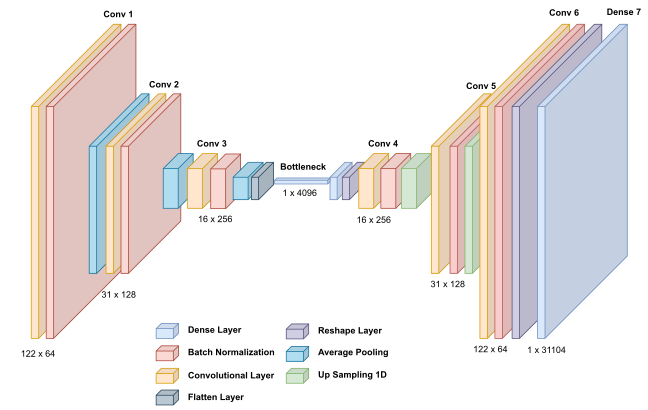
\includegraphics[width=0.5\textwidth]{images/cnn_autoencoder}
	\caption{CNN Autoencoder}
	\label{fig:cnn_autoencoder}
\end{figure}

SGD (Stochastic Gradient Descent) algorithm has been used with a learning rate of $\eta = 0.05$ to train the autoencoder for 1500 epochs with a batch size of 100 (\vref{fig:cnn_autoencoder_loss}), clipping the $L_2$ norm of the gradient to 1 and the value to of weight gradient to 0.5, in order to reduce overfitting and avoid gradient exploding.

Furthermore, as briefly mentioned before, a dropout rate of 0.5 has been applied alongside bottleneck activity regularization to prevent overfitting and make the learned data representations as sparse as possible.

\begin{figure}
	\includegraphics[width=0.5\textwidth]{images/cnn_autoencoder_graph.png}
	\caption{CNN Autoencoder Train/Validation Loss over  the first 500 epochs.}
	\label{fig:cnn_autoencoder_loss}
\end{figure}

Looking at the structure in detail, we will explore layer by layer the structure of the encoder and decoder (excluding dropout layers).

Our model's encoder consists of $3$ convolutional layers with an increasing number of filters, always followed by a batch normalization layer and by an average pooling layer that downsamples the input representation by taking the average value over the window defined by the pool size. The complete set of the encoder parameters is reported in table \vref{tab:cnn_encoder}.

\begin{footnotesize}
	\begin{table}
		\centering
		\caption{Parameters of CNN Encoder}
		\label{tab:cnn_encoder}
		\begin{tabularx}{0.5\textwidth}{XXr}%lMr
			\toprule
			\textbf{Layer Type} & \textbf{Parameters}                                                                   & \textbf{Shape} \\
			\midrule
			Input               &                                                                                       & (1, 243, 128)  \\
			Conv 1D             & \shortstack{\\ Filters, kernel, stride \\(64, 7, 2) \vphantom{space} }                & (122, 64)      \\[0.25cm]
			Batch Normalization & Features = 64                                                                         & (122, 64)      \\[0.25cm]
			Average Pooling     & Pool size = 2                                                                         & (61, 64)       \\[0.25cm] 
			Conv 1D             & \shortstack{\\ Filters, kernel, stride \\(128, 5, 2) \vphantom{space} }               & (31, 128)      \\[0.25cm]
			Batch Normalization & Features = 128                                                                        & (31, 128)      \\[0.25cm]
			Average Pooling     & Pool size = 2                                                                         & (16, 128)      \\[0.25cm]
			Conv 1D             & \shortstack{\\ Filters, kernel, stride \\(256, 5, 1) \vphantom{space} }               & (16, 256)      \\[0.25cm]
			Batch Normalization & Features = 128                                                                        & (16, 256)      \\[0.25cm]
			Average Pooling     & Pool size = 2                                                                         & (8, 256)       \\[0.25cm]
			Flatten Dense       &                                                                                       & (1, 4096)      \\
			\bottomrule
		\end{tabularx}
	\end{table}
\end{footnotesize}

The decoder is very similar to the encoder, but in reverse order, as it reconstructs the encoder’s input based on encoder’s output.

In order to match the dimension of the input, three transposed convolutional layers are needed
in the decoder in combination with upsampling layers that repeats each temporal step $r$ times along the time axis, upscaling the dimension of the reconstructed pattern, and a final triplet composed of reshape, dense and reshape layers. Decoder parameters are reported in Table \vref{tab:cnn_decoder}, while complete model architecture can be visualized in Figure \vref{fig:cnn_autoencoder}.

\begin{footnotesize}
	\begin{table}
		\centering
		\caption{Parameters of CNN Decoder}
		\label{tab:cnn_decoder}
		\begin{tabularx}{0.5\textwidth}{XXr}%lMr
			\toprule
			\textbf{Layer Type} & \textbf{Parameters}                                                                   & \textbf{Shape}    \\
			\midrule
			Dense               &                                                                         				& (1, 4096)         \\[0.25cm]
			Reshape             &                                                                                       & (16, 256)         \\[0.25cm]
			Conv 1D Transpose   & \shortstack{\\ Filters, kernel, stride \\(256, 5, 1) \vphantom{space} }               & (16, 256)         \\[0.25cm]
			Batch Normalization & Features = 256                                                                        & (16, 256)         \\[0.25cm]
			Up Sampling 1D      & Size = 2                                                                              & (32, 256)         \\[0.25cm]
			Conv 1D Transpose   & \shortstack{\\ Filters, kernel, stride \\(128, 5, 2) \vphantom{space} }               & (64, 128)         \\[0.25cm]
			Batch Normalization & Features = 128                                                                        & (64, 128)         \\[0.25cm]
			Up Sampling 1D      & Size = 2                                                                              & (128, 128)        \\[0.25cm]
			Conv 1D Transpose   & \shortstack{\\ Filters, kernel, stride \\(64, 7, 2) \vphantom{space} }                & (256, 64)         \\[0.25cm]
			Batch Normalization & Pool size = 2                                                                         & (256, 64)         \\[0.25cm]
			Reshape             &                                                                                       & (1, 16384)        \\[0.25cm]
			Dense               &                                                                          				& (1, 31104)        \\[0.25cm]
			Reshape             &                                                                                       & (1, 243, 128)     \\
			\bottomrule
		\end{tabularx}
		
	\end{table}
	
\end{footnotesize}